% Created 2020-09-30 Wed 15:22
% Intended LaTeX compiler: pdflatex
\documentclass[10pt,t]{beamer}
\usepackage[utf8]{inputenc}
\usepackage{graphicx}
\usepackage{grffile}
\usepackage{longtable}
\usepackage{wrapfig}
\usepackage{rotating}
\usepackage{textcomp}
\usepackage{amssymb}
\usepackage{capt-of}
\usepackage{hyperref}
\usetheme{default}
%
\usepackage[font=small,labelfont=bf]{caption} % Required for specifying captions
%
\author{C. L. Hepplewhite}
\date{\today}
\title{\large Radiative Transfer Algorithm Updates}
\subtitle{\footnotesize{AIRS Virtual Science Team Meeting}}
\date{\vspace{0.1in}\footnotesize{October 2020 \vfill}}
\author{C. L. Hepplewhite\inst{1,2}, L. Larrabee Strow\inst{1,2}, and S. deSouza Machado\inst{1,2} }
\institute[UMBC]{\inst{1} UMBC Physics Dept. \and \inst{2}UMBC JCET}
\input beamer_setup
\metroset{titleformat title=allcaps}
\setbeamertemplate{frame footer}{UMBC Atmospheric Spectroscopy Lab}
\begin{document}

\maketitle

% -----------------------------------------------------
\begin{frame}{Introduction}
\begin{itemize}
  \item Current and upcoming set of SARTA builds 
  \item Possible future improvements 
  \item Minor fitting improvements
  \item RTA/HITRAN intercomparisons and tuning issues
\end{itemize}

\end{frame}
% ----------------------------------------------------
\begin{frame}{Current Spectroscopy}
  \begin{itemize}
  \item HITRAN 2016
  \item CO2, CH4 line mixing from LBLRTM12.8
  \item MT CKD3.2
  \item CO2 CIA from WV and N2 by Hartmann (4.3 um)
  \item Single parameter surface emissivity.
  \end{itemize}

Used in IASI, AIRS L1c, and CHIRP RTAs.

\end{frame}
% -------------------------------------------------
\begin{frame}{Current SARTAs at ASL}

  \begin{itemize}
  \item The following SARTAs are in use at ASL:
    Dates are release dates.
    \begin{itemize}
    \item AIRS L1B (2008):  Used in AIRS V6, V7 Level 2
    \item AIRS L1C (2019):  Possible use by Bill Irion, CLIMCAPS
    \item CrIS NSR v2012, \& v2016  
    \item CrIS FSR v2016
    \item IASI v2008 and v2016
    \item CHIRP v2020
    \end{itemize}
  \end{itemize}
\end{frame}
% ---------------------------------------------------
\begin{frame}{Future Improvements/Activities}

  \begin{itemize}
  \item HITRAN 2020, should be out this year.
  \item Line Mixing package from the HITRAN (Iouli Gordon, Harvard-Smithsonia).
  \item Currently use kCARTA at 0.0025 cm-1 steps, can move to 0.0005 cm-1 step in 15 \um m region
  \item Interpolation improvements in kCARTA
  \item Nalli surface emissivity parameterization?  Under study.
  \item Improved non-LTE, the extreme solar angles.  Not yet started.
  \item RTA tuning in collabortion with Chris Barnet and Bill Irion (more later in talk)
  \item Hope to perform major re-validation on new RTAs using HITRAN 2020, probably last time...
  \end{itemize}
\end{frame}

% ------------------------------------------------
\begin{frame}[shrink=5]{Validation: Fitting Accuracy}

Here concentrate just on fitting accuracy.  Future work on independent validation using re-analysis, sondes, etc.

  % \begin{itemize}
  % \item After completing the fast coefficient regression, top-of-atmosphere (TOA) radiances predicted by SARTA are compared to those from kCARTA from the training set or extended profile set.
  % \end{itemize}
      \begin{center}
    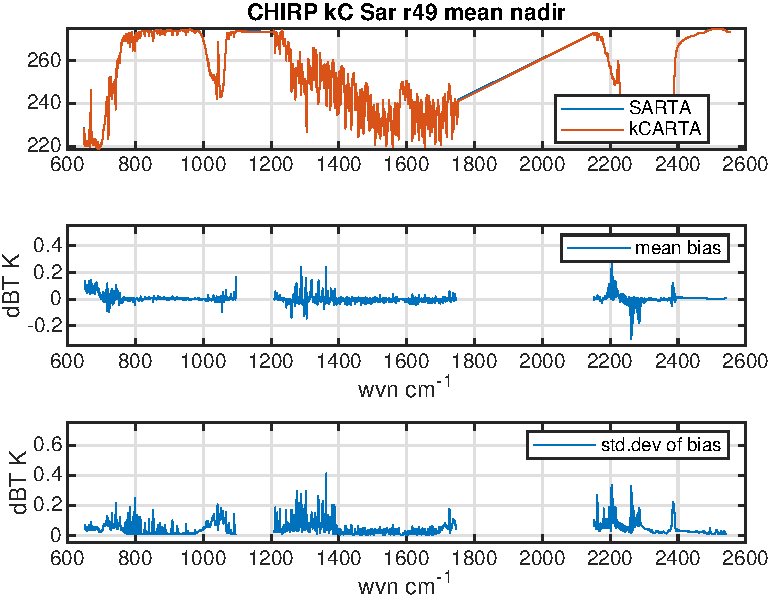
\includegraphics[width=0.6\linewidth]{./Figs/chirp_49regr_sar_kc_bias_stdv.pdf}
    \captionof{figure}{CHIRP bias and std for 49 fitting profiles, 7 secant angles.}
  \end{center}
  

\end{frame}
% -----------------------------------------------
%\begin{frame}[shrink=10]{Improved bias \& std.dev relative to kCARTA}
\begin{frame}{Improved bias \& std.dev relative to kCARTA}

  \begin{itemize}
  \item kCARTA monochromatic layer-so-space optical depths are convolved to the sensor grid.
  \item For AIRS (and any spectrometer) convolution with the spectral response functions (SRF) is well behaved. Transmittance approaches zero for opaque channels.
  \item For interferometers (IASI, CrIS, CHIRP) convolution with the instrument line shape (ILS) produces tau that goes -ve and +ve into the opaque region.
  \item Regression of the fast coefficients is controlled down to a minimum transmittance which is set by inspection of these 'wings'.
  \item Sarta builds for IASI, CrIS version 2019 and CHIRP 2020 included some fits in strong (CO2) bands that were not optimal. (See next slides).
  \end{itemize}

\end{frame}

% -----------------------------------------------
\begin{frame}{Example of optimization: CHIRP 640 cm-1}

  \begin{center}
    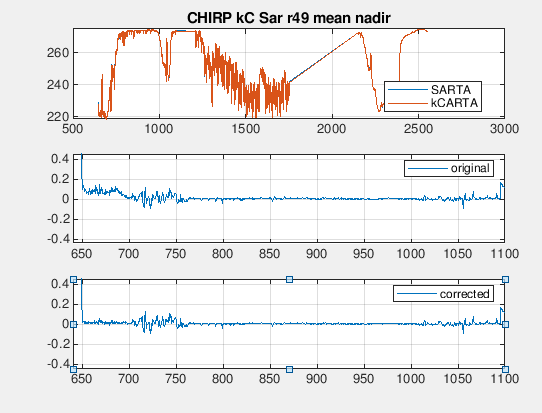
\includegraphics[width=0.6\linewidth]{./Figs/chirp_optimize1.png}
    \captionof{figure}{CHIRP SARTA bias compared to kCARTA, with and without improved regression.}
  \end{center}


\end{frame}
% -----------------------------------------------
\begin{frame}[shrink=5]{Example of optimization: IASI 2300 cm^{-1}}

\vspace{-0.5cm}
  \begin{center}
    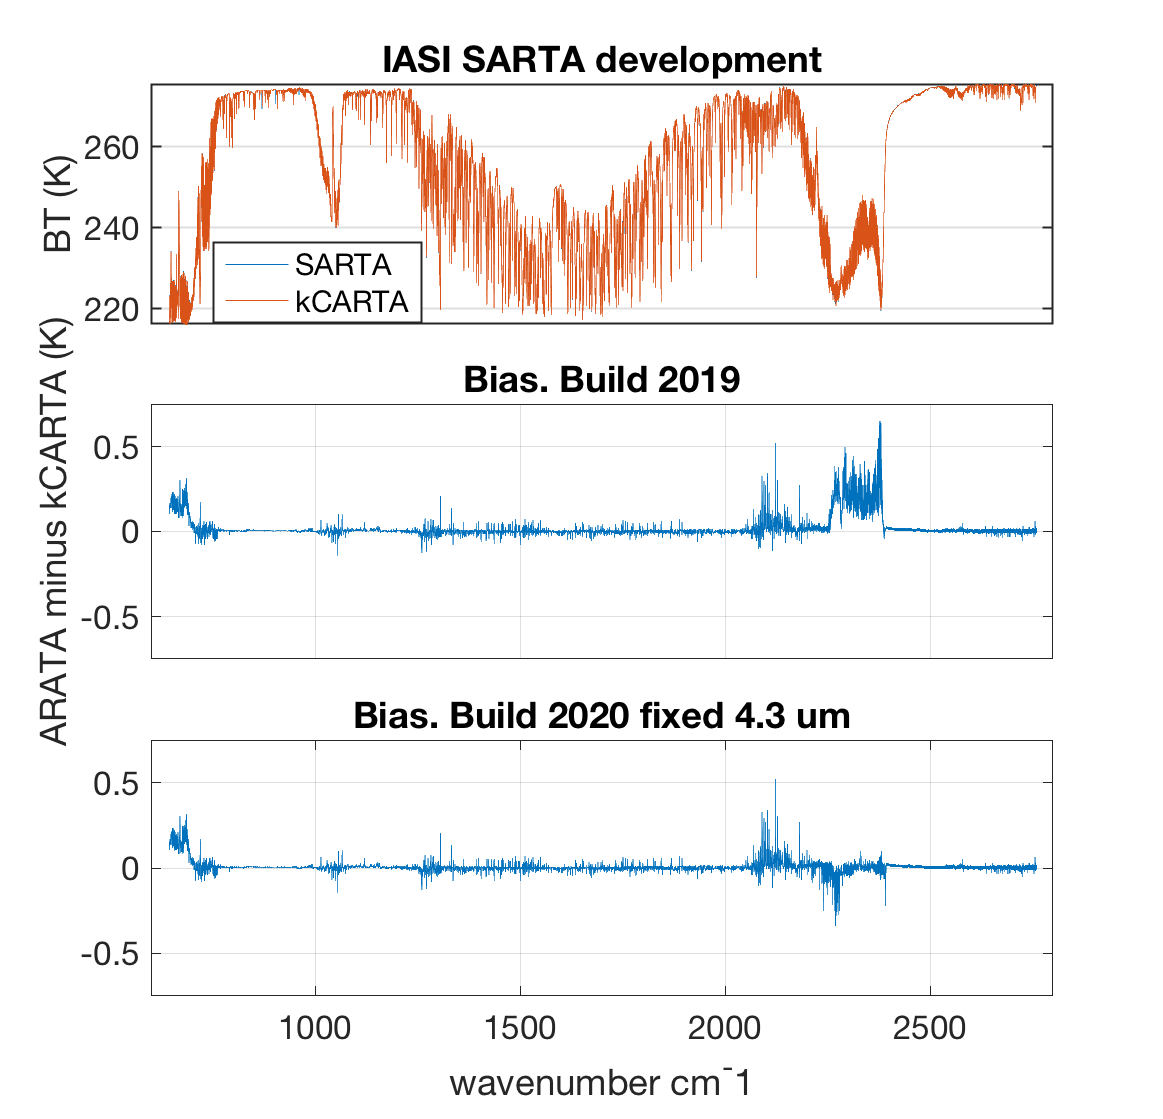
\includegraphics[width=0.6\linewidth]{./Figs/iasi_sarta_kcarta_mean_bias_4p3um_fx.png}
    \captionof{figure}{IASI SARTA bias compared to kCARTA, with and without improved regression at 4.3 um.}
  \end{center}

\end{frame}
% -----------------------------------------------
\begin{frame}{Tuning}

  \begin{block}{}
  Retrieval and NWP assimilation require Obs - Fit bias removal, via ``tuning'' Bias can occur because of:  
  \end{block}
    
  \begin{itemize}
  \item AIRS radiometric calibration.
  \item AIRS spectral calibration and instrument line shape.
  \item AIRS fast model parameterization.
  \item Spectroscopy (including continuum and lineshape)
  \item Cloud contamination in fields of view selected as clear
  \item Validation data, including time/space mismatches and uncertainties in minor gas abundances.
  \end{itemize}

Two approaches: (a) Tune the spectroscopy (optical depths), (b) Tune the (Obs - Calc) B(T)'s.
  
\end{frame}
% -----------------------------------------------
% \begin{frame}{Tuning: 2}

%   \begin{block}{}
%     The objective of tuning is to reduce bias in the real world sufficiently to increase the yield in single footprint geophysical retrievals.
%   \end{block}

%   \begin{itemize}
%   \item Large data sets are compared covering all global atmospheric and scene types.
%   \item Bias and std.dev characterisctics between coincident TOA measurements with forward model predictions are determined.
%   \item RTA transmittances are adjusted for specific channels where needed.
%   \item SARTA uses a supporting data file of tuning parameters.
%   \item Tuning of transmittances in the RTA are preferred over tuning BT of TOA predicts.

%   \end{itemize}

% \end{frame}
% ----------------------------------------------
\begin{frame}{Tuning: Case study}

  \begin{block}{}
  \end{block}

  \begin{itemize}
  \item Selection of June 25 talk
  \end{itemize}

\end{frame}
% ----------------------------------------------
\begin{frame}{Conclusions}

  \begin{block}{}
  \end{block}

  \begin{itemize}
  \item RTA (kCARTA and SARTA) development and maintenance continues at UMBC/JCET.
  \item SARTA for AIRS, CrIS (NSR FSR), IASI and CHIRP have been or are being developed, tested
    and verified.
  \item CHIRP SARTA is in progress.
  \item Tuning for builds from 2019 are either partial or pending.
    
  \end{itemize}

\end{frame}
% -----------------------------------------------


\end{document}


% -----------------------------------------------------
\begin{frame}{The SARTA}

  \begin{itemize}
  \item The Stand-alone radiative transfer algorithm (SARTA) is constructed using kCARTA
  \item Therefore SARTA has the same spectroscopy as kCARTA.
  \item SARTA was developed 18 years ago for the AIRS.
  \item It uses sets of coefficients that parameterize atmospheric transmittances derived using a set of training profiles.
  \item Is written in Fortran
  \item Permits very fast computation of radiances for predefined spectral response functions.
    \item Has a version for clear sky radiance calculations and for cloudy radiances.
    
\end{itemize}

\end{frame}
% ----------------------------------------------------
\begin{frame}{Who uses SARTA}

  \begin{itemize}
  \item SARTA is used to compute clear and all-sky radiances for any and all FoVs from AIRS, CrIS and IASI missions.
  \item Is fast enough to make whole-mission modelling easily manageable. Faster than kCARTA *way* faster than LBL.
  \item Currently used in ASL for the RTP production for analysis of sensor performance and global studies and geophysical retireval.
  \item Is used in the AIRS geophysical product retrieval.
    \item Is used in NUCAPS.

  \end{itemize}
\end{frame}

%%% Local Variables:
%%% mode: latex
%%% TeX-master: t
%%% End:
